\section{Evaluation datasets}



To validate the industrial solution beforehand on comprehensive dataset we use following as a benchmark.  Faults in the wild are rare so the preparation of balanced datasets is done create deficient configuartions on purpose. Datsets MaFaulDa and CWRU bearing dataset are being used in related work and are publically available in the Comma-Separated Values format. There is also less comprehensive dataset conserning unbalance, but demostrates behaviour during revolution speed up.  

\subsection{Machinery Fault Database}
(MaFaulDa)
50 kHz, 5 sec. recordings, 
Rotation speeds 10~Hz - 60~Hz (737 rpm - 3686 rpm with steps of approximately 60 rpm)

% Sensors: 
	% - Accelerometers IMI 601A01/604B31,  Range ±50 g (±490 m/s2)
	% Magnetic tachometer MT-190
	% Shure SM81 microphone with frequency range of 20-20.000 Hz
	% National Instruments NI 9234 4 channel analog acquisition modules, with sample rate of 51.2 kHz 

% Normal
% Imbalance  - load values within the range from 6 g to 35 g (step of 5g)
% Misalignment (Horizontal/Vertical)
% Bearings (Overhang / Underhang) - Inner, Outer, Cage

% total of 1951 different fault scenarios for 4 different operational conditions. 
% 49 of which from the normal class, 333 from unbalance class, 498 from misalignment class and 1071 from the bearing fault.

% 2 sets of accelerometers each one associated to one bearing (inner and outer) and measuring in 3 directions

% Column 1 - tachometer signal that allows to estimate rotation frequency
% Columns 2 to 4 - underhang bearing accelerometer (axial, radiale tangential direction)
% Columns 5 to 7 - overhang bearing accelerometer (axial, radiale tangential direction)
% Column 8 - microphone


RotorKit Alignment Balance Vibration Trainer (ABVT)
\cite{pestana-viana_influence_2016}
\cite{ribeiro_rotating_2017}

 \footnote{\url{https://www02.smt.ufrj.br/~offshore/mfs/page_01.html}}

\begin{figure}[h]
\centering
\begin{subfigure}[b]{0.48\textwidth}
	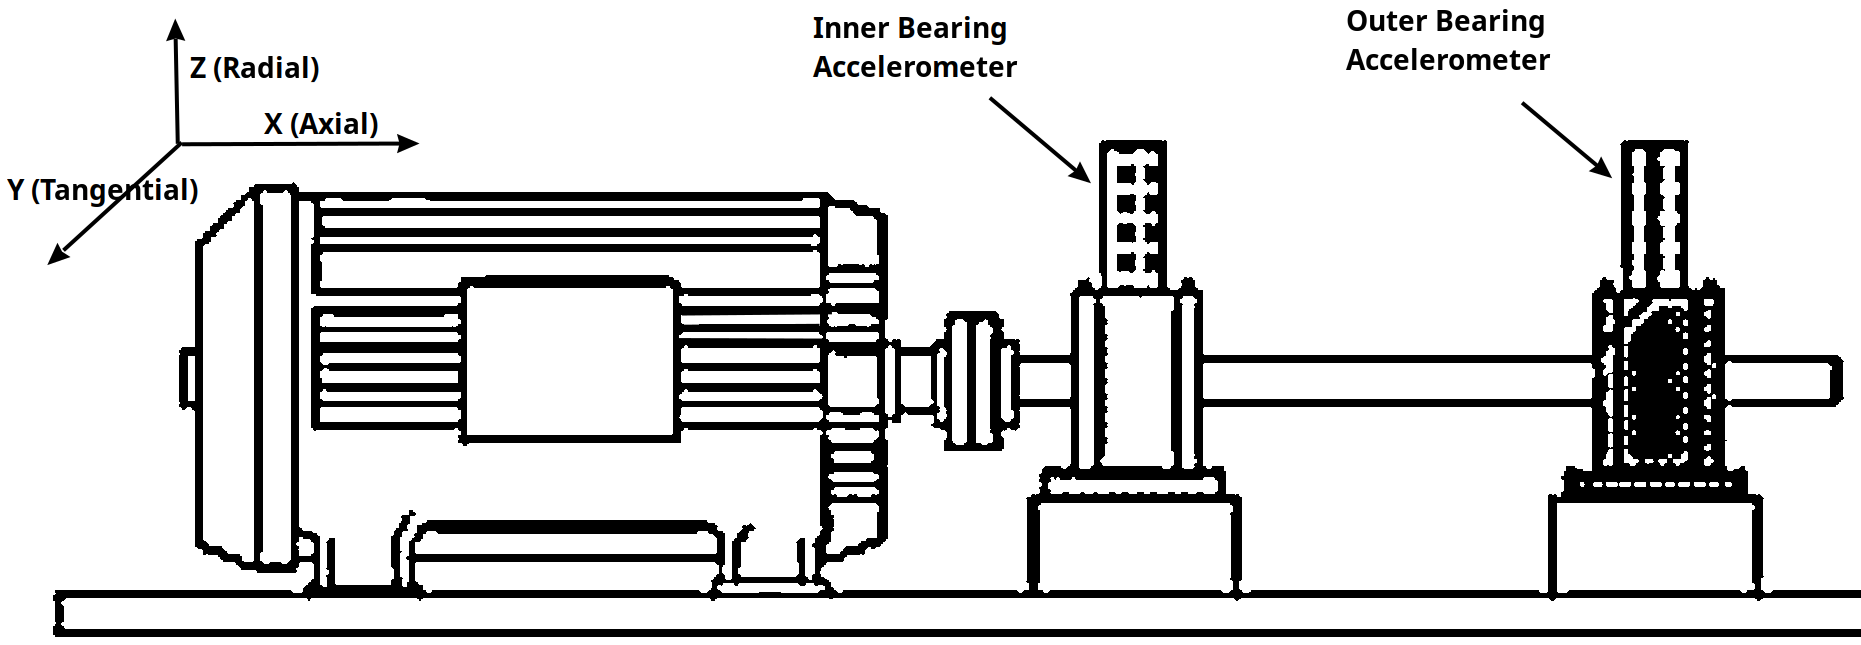
\includegraphics[width=\textwidth]{assets/mafaulda-simulator.png}
	\caption{Schematic diagram \cite{pestana-viana_influence_2016}}
\end{subfigure}
\hfill
\begin{subfigure}[b]{0.48\textwidth}
	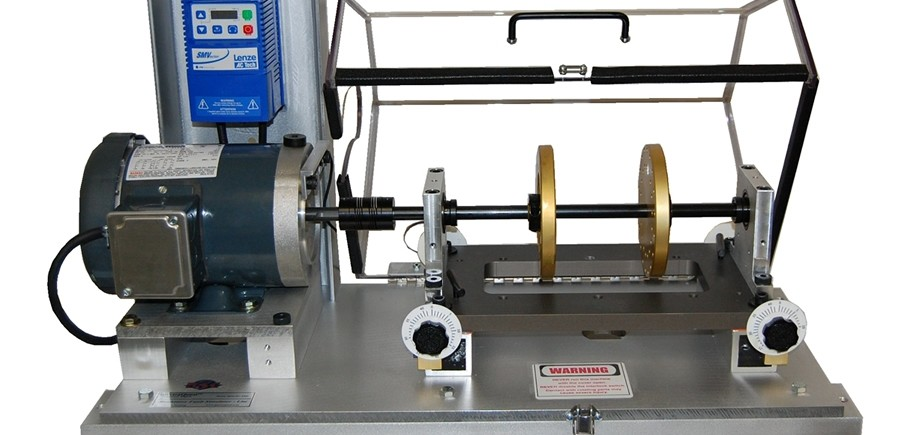
\includegraphics[width=\textwidth]{assets/machinery-fault-simulator.jpg}
	\caption{Mechanical construction \cite{noauthor_spectraquest_nodate}}
\end{subfigure}
\caption{Machinery Fault Simulator for MaFaulDa}
\label{fig:mafaulda-simulator}
\end{figure}



\subsection{Case Western Reserve University bearing database}
(CWRU) 
2 HP (1.492 kW) Reliance Electric motor \footnote{\url{https://engineering.case.edu/bearingdatacenter/download-data-file}}
Bearings - Inner, Outer
12 kHz, 48 kHz
fan and drive end bearings
Fault diameters of 7 mils, 14 mils, 21 mils, 28 mils, and 40 mils (1 mil=0.001 inches) in diameter were introduced separately at the inner raceway, rolling element (i.e. ball) and outer raceway. 

% Faults ranging from 0.007 inches in diameter to 0.040 inches in diameter were introduced separately 
% at the inner raceway, rolling element (i.e. ball) and outer raceway. 
%Faulted bearings were reinstalled into the test motor and vibration data
%was recorded for motor loads of 0 to 3 horsepower (motor speeds of 1797 to 1720 RPM).

% Feature-based performance of SVM and KNN classifiers for diagnosis of rolling element bearing faults
\cite{jamil_feature-based_2021}

\begin{figure}[h]
\centering
\begin{subfigure}[b]{0.48\textwidth}
	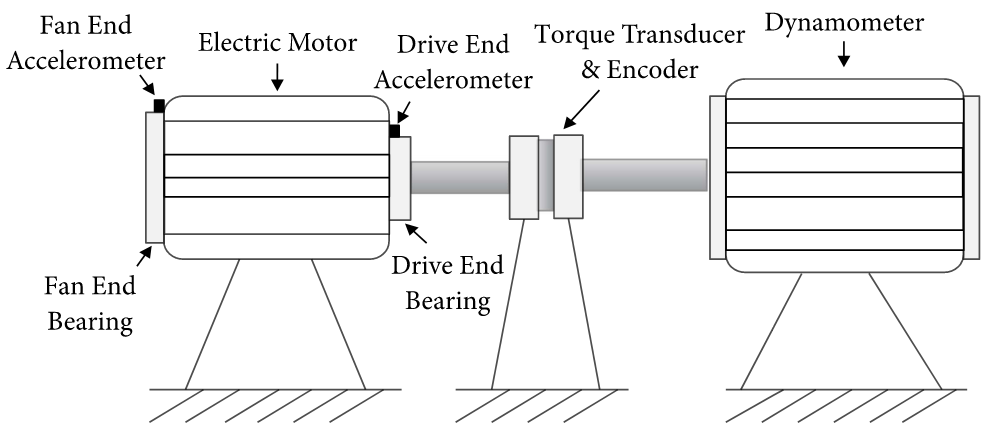
\includegraphics[width=\textwidth]{assets/cwru-test-stand-2.png}
	\caption{Schematic diagram \cite{song_bearing_2022}}
\end{subfigure}
\hfill
\begin{subfigure}[b]{0.48\textwidth}
	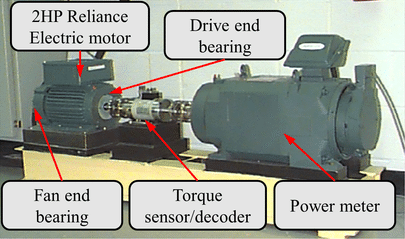
\includegraphics[width=\textwidth]{assets/cwru-test-stand.png}
	\caption{Mechanical construction \cite{yuhong_new_2021}}
\end{subfigure}
\caption{CWRU apparatus}
\label{fig:cwru-simulator}
\end{figure}



\subsection{Unbalance on rotating shaft}
Shaft -  unbalances of different sizes \footnote{\url{https://www.kaggle.com/datasets/jishnukoliyadan/vibration-analysis-on-rotating-shaft}}

% Unbalances of different sizes was recorded. Sampling rate =  4096 Hz
% 4 different unbalance strengths were recorded as well as one dataset with the unbalance holder without additional weight (i.e. without unbalance). 
%The rotation speed was varied between approx. 630 and 2330 RPM in the development datasets 
% and between approx. 1060 and 1900 RPM 

%Columns:
% V_in =  The input voltage to the motor controller V_in (in V)
% Measured_RPM  = The rotation speed of the motor (in RPM; computed from speed measurements using the DT9837)
% Vibration_[1 - 3]      : The signal from the 1.,2.,3. vibration sensor

% (“0” = no unbalance, “4” = strong unbalance), (“D” = development or training, “E” = evaluation)
% Radius in mm = 0, 14, 18.5, 23, 23
% Mass 3.3 g (0 ... 3), 6.6 g in 4

\begin{figure}[h]
\centering
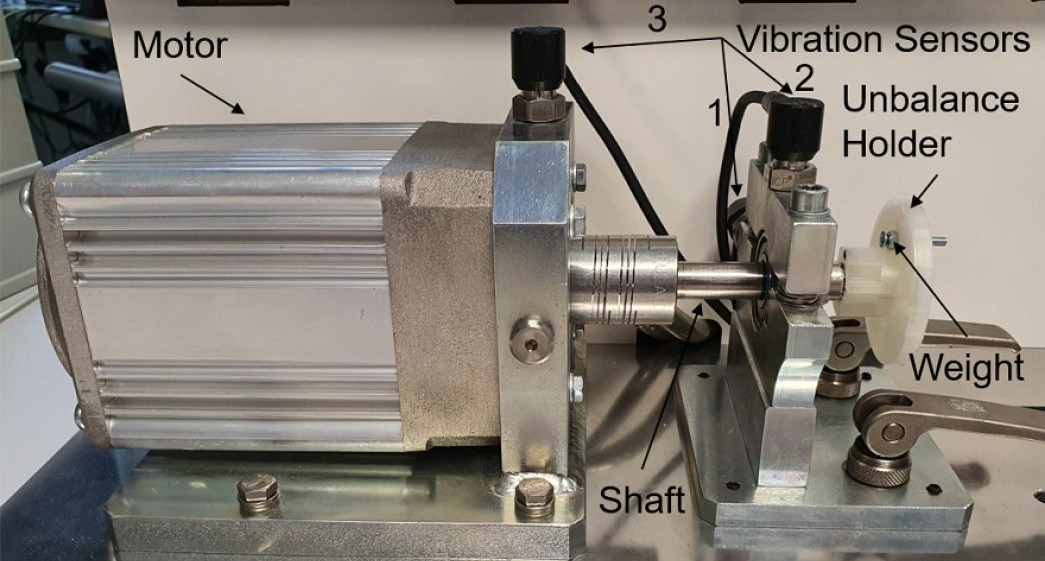
\includegraphics[width=0.7\textwidth]{assets/rotating-shaft.jpg}
\caption{Rotating shaft dataset \cite{mey_machine_2020}}
\label{fig:rotating-shaft}
\end{figure}

% Machine Learning-Based Unbalance Detection of a Rotating Shaft Using Vibration Data
\cite{mey_machine_2020}

